\documentclass{lni}


\IfFileExists{latin1.sty}{\usepackage{latin1}}{\usepackage{isolatin1}}
\usepackage{graphicx}
\usepackage{url}
\usepackage{listings}
\usepackage{nameref}
\graphicspath{{pix/}{}}

\author{Gerhard Gr?schl, Miran Mizani\\\{gerhard.groeschl, miran.mizani\}@campus.lmu.de\\\\
Seminar: Trends in Mobilen und Verteilten Systemen \\Wintersemester 2016/2017\\\\
Lehrstuhl f?r Mobile und Verteilte Systeme\\Institut f?r Informatik\\Ludwig-Maximilians-Universit? M?nchen\\\\
Betreuer: Michael T. Beck\\\textit{eingereicht am \today}}
\title{Sicherheitsaspekte bei Deployment virtueller Netzwerkinfrastrukturen}



\begin{document}
\maketitle

\vfill
FEHLT [GG]: Optimierung der Grafiken, Erkl?ung der Ansatz2-Algorithmen, Ansatz2 Komplexit? und Performanz, Vergleich, Einf?bung der Gleichung Ansatz1, Legende maMo Ansatz2

FRAGEN[GG]: mathematische Modelle rausnehmen?

\begin{abstract}
Durch die ??rst effiziente Nutzung von Hardware mittels Virtualisierung steigt die Nachfrage nach virtualisierten Infrastrukturen enorm. Serviceprovider m?ssen die Hardwarebasis f?r ihre Dienste nicht mehr selbst unterhalten und geben ihre dahingehende Verantwortung an Infrastrukturanbieter weiter. Um die Sicherheit dieser Strukturen nicht zu vernachl?sigen, arbeiten viele Forscher in diesem Bereich und versuchen effiziente Algorithmen mit integrierter Beachtung der Sicherheitsaspekte zu finden. Diese Arbeit soll einen ?erblick und eine Klassifizierung der Gefahren, die solche Konstrukte betreffen, sowie eine Analyse zweier unterschiedlicher Ans?ze zur Vermeidung m?glichst vieler Risiken zum Zeitpunkt der Planung ?bermitteln.
%Hier folgt eine kurze Zusammenfassung des Themas sowie der wichtigsten Erkenntnisse und Ergebnisse. L?ge: ca. 200 W?rter.
\end{abstract}


\newpage
\tableofcontents
\newpage

\section{Einleitung}
\label{sec:Einleitung}
%Internet impasse
Ein Konzept dem Internet Impasse mit flexibler Architektur \underline{[WAS IST DAS?]} und Handhabbarkeit zu begegnen, wurde in der Netzwerkvirtualisierung (NV) gefunden. \cite{anderson2005overcoming, bays2012security, fischer2013virtual} Sie basiert auf Knoten- (z.B. Xen) und Linkvirtualisierung \underline{[ANGABE ZU BEIDEM?]} und erlaubt so von der tatsächlichen physischen Hardware und Netzinfrastruktur (NI) beinahe unabhängige logische bzw. virtuelle Netzwerke einzurichten, welche nach außen hin den Anschein physischer Netzwerke erwecken. Die Möglichkeit mehrere virtuelle Maschinen (VMs) pro physischem Host und verschiedene heterogene virtuelle Netzwerke (VNs) auf demselben physischen Substratnetz zu betreiben befördert die Flexibilität der Netzwerkarchitektur und wirkt dem Internet Ossification Problem \cite{anderson2005overcoming} entgegen.

%Vorteile von NV
Die großen Vorteile der NV liegen in der Abstraktion von der eingesetzten Hardware. Das Erstellen, Verändern, Migrieren, Zurücksetzen und Löschen von Maschinen funktioniert genauso einfach wie der Umgang mit Dateien, was eine dynamischere Nutzung des Netzwerkes erlaubt. Virtuelle Maschinen und Netzwerke eigenen sich auch als Testumgebung. Einerseits werden bestehende Systeme im Fehlerfall nicht direkt beeinträchtigt. Andererseits kann neuer Code nun leicht in verschiedenen Umgebungen (Windows, Linux, verschiedengroßer RAM, mit oder ohne Software-Developer-Kits etc.) ohne zusätzliche Hardware getestet und später einfach ausgerollt werden.

NV eröffnet eine Unterteilung des klassischen Internetserviceproviders (ISP) in Service-Provider (SP) und Infrastructure-Provider (InP). Damit gewonnene Freiheiten durch z.B. jeweils unabhängige Technologieentscheidungen[wang2016towards] sind wohl besonders für Unternehmen interessant, die die Hardwarebasis ihrer Dienste nicht mehr selbst unterhalten wollen.\\
Das Anbieten von Software und Hardware als on-demand Ressourcen wird wegen geringeren Wartungsaufwand, verminderte Hardwarekosten durch Koexistenz mehrerer Mieter, aber v.a. wegen Automatisierbarkeit in der Programmierung der Netzwerkumgebung vereinfacht. Dass InPs nicht mehr streng durch Hardware limitiert sind, begünstigt Skalierbarkeit und bspw. lastbedingte Migration von VMs auf andere physische Hosts.\\
Auch für den Kunden bietet NV Vorteile: Unternehmen bezahlen nur noch für diejenigen Ressourcen, die gerade in Anspruch genommen werden. Hochqualitative Hardware kann so zu einem Bruchteil ihres Preises erworben und ungenutzte Hardware reduziert werden. Durch dynamisches Skalieren (z.B. in Zeiten hoher Last) kann die eigene IT-Landschaft mühelos vergrößert werden.

%Ziele von NV
Das Outsourcing von Rechenleistung, Speicher, Inhalten und Netzwerk soll Soft- und Hardware einfacher nutzbar machen und Geschäftsprozesse befördern. Die damit einhergehende Verantwortungsübertragung erfordert eine Anpassung des Risikomanagements und IT-Sicherheitstechnische Arbeiten zur Erhaltung der klassischen C.I.A.-Aspekte. Wegen der gemeinsam genutzten Hardware kommt aus Sicht des Kunden besonders der Isolation und dem Datenschutz eine wichtige Rolle zu.\\
Bekannte Sicherheitsmechanismen wie Verschlüsselung, Firewalls, Intrusion Detection Systeme etc. können zwar auf den virtuellen Komponenten des Netzwerks implementiert werden. Die Sicherheit von Nutzerdaten könne dadurch aber wegen der heterogenen und stark dynamischen Struktur virtueller Umgebungen jedoch nicht garantiert werden. Ferner dürften Vorteile der Netzwerkvirtualisierung durch den zusätzlichen Overhead verloren gehen. \cite{gong2016virtual}\\
Eine mögliche Lösung hierzu ist das Integrieren von Sicherheitsaspekten bereits in die Zuordnung von virtuellen zu physischen Knoten und Links. Dieser Virtual Network Embedding (VNE) Prozess stellt eine der größten Herausforderungen in der Netzwerkvirtualisierung dar. \cite{fischer2013virtual}
Werden virtuelle Netzwerke entsprechend ihrer Sicherheitsanforderungen bereits auf Substratknoten mit hinreichender Schutzfunktion wie beispielsweise Firewall abgebildet, so kann Overhead durch zusätzliche Sicherheitstechnik im laufenden Betrieb des VNs reduziert werden.

[TODO]
Derzeit wird versucht \cite{bays2012security, gong2016virtual, wang2016towards} derartige Probleme bereits im VNE-Algorithmus anzugehen [SVNE Security-aware VNE|security by design]. Nicht allen Problemen bzw. Sicherheitsrisiken kann aber auf diese Weise begegnet werden. %(= Überleitung zur Gliederung und zweiten Kapitel?)


Diese Arbeit soll Gefahren im Kontext virtualisierter Netzwerke klassifizieren und zwei unterschiedliche Ansätze zur Schaffung eines möglichst hohen Sicherheitsniveaus bereits zum Zeitpunkt des VNE-Prozesses analysiert.\\
Dazu wird zuerst das VNE-Problem in Kapitel \ref{sec:VNE-Problem} \textit{\nameref{sec:VNE-Problem}} dargestellt. Kapitel \ref{sec:gefahren} \textit{\nameref{sec:gefahren}} untersucht Sicherheitsanforderungen an virtuelle Netzwerkstrukturen und klassifiziert Sicherheitsrisiken, die sich in deren Kontext ergeben. Zwei Möglichkeiten zur Vermeidung von Gefahren, denen bereits im VNE-Prozess begegnet werden kann, werden im Kapitel \ref{sec:svne} \textit{\nameref{sec:svne}} betrachtet. Nach einer Diskussion in dieser Arbeit offengebliebener Probleme in Kapitel \ref{sec:offenefragen} \textit{\nameref{sec:offenefragen}} wird mit einem Ausblick abgeschlossen.
[KAPITELNAMEN-REFERENZIERUNG NÖTIG? LIEBER OHNE?]



% Die Ausarbeitung zum Seminar soll dem Layout der \textit{GI-Edition Lecture Notes in Informatics (LNI)} entsprechen. Die verwendete Literatur wird in der beiliegenden Datei \verb+literatur.bib+ verwaltet. Eine Referenz kann mittels des \verb+\cite{}+--Kommandos eingef?gt werden, z.B.

% \subsection{Hinweise f?r Abbildungen}
% Abbildungen m?ssen als \texttt{.pdf}, \texttt{.png}, oder \texttt{.jpg} eingebunden werden. Beispiel:
% \begin{figure}[htb]
%   \begin{center}
%     
\includegraphics[width=1cm]{gilogo.pdf}
%     \caption{\label{logo}Das Logo der GI}
%   \end{center}
% \end{figure}


\section{Das Virtuel Network Embedding Problem}
\label{sec:VNE-Problem}
Um den Anforderungen der heutigen Gefahren zu gen?gen, ist es unumg?glich s?tliche Grunds?ze der IT-Sicherheit m?glichst fr?h in die Planung der gew?nschten Infrastruktur miteinzubeziehen. Nicht nur, weil das nachtr?liche Schlie?n von Sicherheitsl?cken und Hinzuf?gen von Sicherheitskomponenten in finanzieller und zeitlicher Hinsicht zehnmal so teuer ist wie die initiale Beachtung dieser Aspekte, sondern weil die vollst?dige Sicherheit eines nachger?steten Systems kaum gew?rleistet werden kann \cite{Cole}."`Security-by-Design"' ist einer der wichtigsten Begriffe bei der Planung ?ffentlich zug?glicher Netzwerkstrukturen. Dementsprechend gro?ist die Nachfrage nach VNE-Algorithmen, die bereits beim Prozess des Mappings m?glichst viele Sicherheitsaspekte beachten und abdecken. Die vorausgehende Klassifizierung der bekannten Gefahren in "`VNE-relevant"' und "`nicht-VNE-relevant"' bildet die Grundlage f?r unsere weiteren Untersuchungen. Um zuvor noch einen genaueren Einblick in die Problematik von VNE zu gew?ren, beginnen wir zun?hst mit der Erl?terung des VNE-Problems sowie einem ?erblick ?ber die verschiedenen erfolgreichen Strategien bestehender VNE-Algorithmen, welche die Sicherheitsaspekte noch nicht beachten. 

Betrachtet man das zugrundeliegende physische System als einen ungerichteten Graphen
\begin{center}
	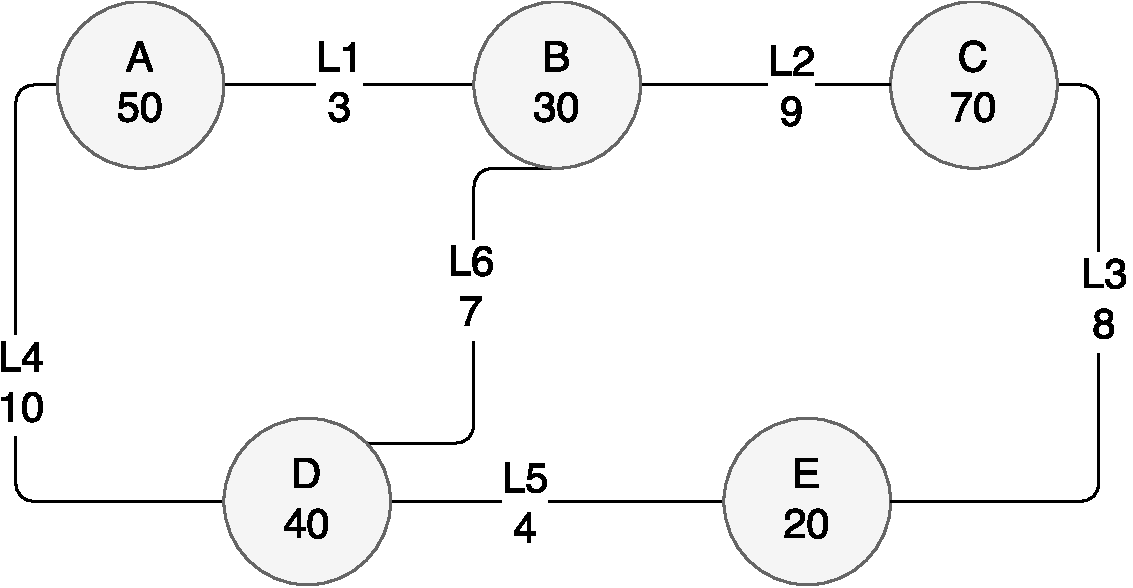
\includegraphics[width=0.7\textwidth]{physical_structure2.pdf}\newline
	  % \caption{\label{logo}(A bis E benennt die Knoten, L1 bis L6 benennt die Links, die Zahlen darunter stehen f?r die jeweiligeverf?gbare Resourcenmenge(abstrakt))}
\end{center}
\vspace*{1cm}

%Grafik
und extrahiert die vorhandenen Elemente sowie deren Werte, erh?t man die Basismenge
\begin{center}
G\textsuperscript{S} = \{N\textsuperscript{S}, L\textsuperscript{S}\}\newline

(N steht f?r die Menge der physischen Knoten, L f?r die Menge der physischen Links)
\end{center}

\begin{center}
G\textsuperscript{S} = 
\{\{
(A\textsuperscript{S},50),(B\textsuperscript{S},30),(C\textsuperscript{S},70),
(D\textsuperscript{S},40),(E\textsuperscript{S},20)\},
\newline\{
(L1\textsuperscript{S},3),(L2\textsuperscript{S},9),(L3\textsuperscript{S},8),
(L4\textsuperscript{S},10),(L5\textsuperscript{S},4),(L6\textsuperscript{S},7)\}\}
\end{center}
in welche die virtuellen Strukturen eingebettet werden sollen.

Ein "`virtual network request"' (in Folge "`VNR"' genannt) kann hierbei ebenfalls als ein ungerichteter Graph gesehen
\begin{center}
	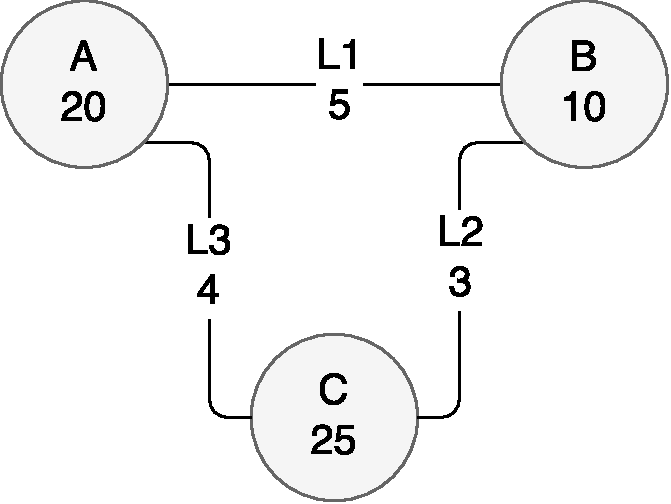
\includegraphics[width=0.4\textwidth]{VNR1.pdf}\newline
	  % \caption{\label{logo}(A bis E benennt die Knoten, L1 bis L6 benennt die Links, die Zahlen darunter stehen f?r die jeweiligeverf?gbare Resourcenmenge(abstrakt))}
\end{center}
%Grafik
und genauso in eine Menge ?bersetzt werden.\newline
\begin{center}
G\textsuperscript{V} = \{N\textsuperscript{V}, L\textsuperscript{V}\}\newline
(N steht f?r die Menge der virtuellen Knoten, L f?r die Menge der virtuellen Links)
\end{center}

\begin{center}
G\textsuperscript{V} = \{\{
(A\textsuperscript{V},20),(B\textsuperscript{V},10),(C\textsuperscript{V},25)\} , \{
(L1\textsuperscript{V},5),(L2\textsuperscript{V},3),(L3\textsuperscript{V},4)\}\}
\end{center}

\begin{center}
Gesucht ist nun eine Abbildungsfunktion f : G\textsuperscript{V} $\rightarrow$ G\textsuperscript{S}
\end{center}

In der Regel ist es ?blich, nicht nur eine einzelne VNRs auf ein physisches System abzubilden, sondern gleich mehrere auf einmal. Ebenso w?e es theoretisch m?glich, dass ein Infrastruktur-Provider gleich mehrere getrennte unabh?gige physische Strukturen betreibt, und somit mittels VNE das beste System f?r die Abbildung der Menge von VNRs eroiren m?chte. Dies k?nnte beispielsweise der Fall sein, wenn ein Serviceprovider ein VNR mit der Bedingung "`alle Elemente m?gen sich am selben Standort befinden, egal an welchem"' in Auftrag gibt, und der Infrastruktur-Provider ?ber mehrere Hardware-Standorte verf?gt.
\newline
% Gv=...
Die Attributmenge bei den grundlegenden VNE-Algorithmen beschr?kt  sich zumeist auf Rechnerleistung und Bandbreite. 
Lokalit?, GPU-Leistung und RAM-Menge w?en einige weitere m?gliche Standard-Attribute. Ein gro?s Problem bei der Berechnung des optimalen Mappings findet sich bei der Berechnungszeit. Die endliche Beschr?kung der Knoten- sowie Link-Resourcen und die "`on-line nature"' von VNRs stellen zus?zliche Hindernisse dar. Da selbst L?sungen f?r einfache Anfragen (geringe Anzahl von Knoten und Links), welche wenige Attribute beinhalten, exponentiellen Rechenaufwand ben?tigen, steigt der Aufwand sowohl mit der Anzahl der abzubildenden Knoten und Links, als auch mit steigender Attributanzahl dementsprechend. Teilweise gilt das Problem als rechnerisch unl?sbar, grunds?zlich aber befinden wir uns im Komplexit?sbereich der NP-Vollst?digkeit \cite{SVNE2}. Da die Erh?hung der Attributmenge - wie bereits genannt - grunds?zlich nicht positiv zur Laufzeit der existierenden Algorithmen beitr?t, werden wir den Komplexit?sbereich beim Hinzuf?gen von Sicherheitsanforderungen nicht verlassen. Dennoch gibt es M?glichkeiten, die den Rechenaufwand reduzieren k?nnen. Im Folgenden widmen wir uns allerdings zuerst einer ?ersicht ?ber die Gefahren, welche bei VNE eine Rolle spielen.



\section{Sicherheitsaspekte virtueller Netzwerk-Infrastrukturen / -systeme}
\label{sec:gefahren}

\subsection{Sicherheitsanforderungen}
\label{subsec:gefahren_anforderungen}
Dummytext. :)

\subsection{Herk?mmliche Gefahren in Netzinfrastrukturen}
\label{subsec:gefahren_allg}



\subsection{Neue Verwundbarkeiten in virtualisierten Umgebungen}
\label{subsec:gefahren_virt}
Dummytext. :)


\subsubsection*{Technischer Art}
\label{subsubsec:gefahren_virt_technisch}
Dummytext. :)

\paragraph{von NI}
\label{parag:vonNI}
bla bla

\paragraph{von VN/VM}
\label{parag:vonVN}
bla bla

\paragraph{von User}
\label{parag:vonUser}
bla bla


\subsubsection*{Organisatorischer Art}
\label{subsubsec:gefahren_virt_organisatorisch}
Dummytext. :)

\subsubsection*{Rechtlicher Art}
\label{subsubsec:gefahren_virt_rechtlich}
Dummytext. :)



\subsection{VNE-Relevante Gefahren}
\label{subsec:gefahren_vnerelevant}	


\section{Vermeidung von Gefahren via Secure VNE (SVNE)}
\label{sec:svne}
Da wir nun einen ?erblick zu VNE sowie den bestehenden Gefahren gegeben haben, widmen wir uns nun zwei verschiedenen SVNE-L?sungsans?zen.

\subsection{Ansatz 1}

Hierbei besch?tigen wir uns mit dem L?sungsansatz aus \cite{wang2016towards}. 
Das Hauptaugenmerk bez?glich der Sicherheitsaspekte legen Wang et al auf Traffic-Verschl?sselung und die Separierung von VMs unterschiedlicher Trust-Levels. Mittels"`Security plan design"'werden die drei folgenden strukturellen Aspekte betrachtet und in dementsprechende Levels eingeteilt.
\begin{itemize}
\item The Network plan:\newline
Ein VNR wird als Netzwerk betrachtet und seinem Level entsprechend isoliert. "`High"'fordert und beansprucht ein gesamtes Netz bzw. Subnetz der physischen Infrastruktur f?r sich. Hiermit soll die Wahrscheinlichkeit f?r DOS-Angriffe oder ?nliche vermindert werden, da"`Mehr-Parteien-Netzwerke"'die Hauptschwachstellen f?r solche Angriffe darstellen \cite{DOS}. Auch Sniffing durch kompromittierte Hosts im selben Netz wird durch diese Ma?ahme verhindert. W?rend "high"'Resourcenteilung somit komplett verweigert, l?st der Level"`medium"'zumindest ein gemeinsam genutztes Netz f?r VNRs vom selben Eigent?mer zu.

\item The Node plan:\newline
Die einzelnen virtuellen Knoten eines VNR stellen Isolierungsanforderungen an die physischen Knoten. Wie auch beim"`network plan", werden die Levels"`high","`medium"'und"`none"'definiert und umgesetzt."`high"'fordert die alleinige Existenz eines VNR-Knotens,"`medium"'l?st VNR-Knoten vom selben Eigent?mer auf ein und demselben physischen Knoten zu. Durch diesen Plan sollen Angriffe von VM zu VM ?ber gemeinsam genutzte Resourcen unterbunden werden. Zus?zlich wird das Risiko eines Angriffs vom physischen Host verringert, da der Angriffsvektor"`VM zu physischem Host"'eliminiert wird.

\item The Link plan:\newline
End-to-End(E2E), Point-to-Point(P2P) und"`none"'sind die hier w?lbaren Levels. W?rend E2E nur an den Endpunkten Verschl?sselungskapazit?en zu Verf?gung stellen muss, ben?tigt P2P diese Kapazit?en an allen Hops des abgebildeten Links. Die heutzutage sehr g?gigen man-in-the-middle Angriffe sollen dadurch wesentlich erschwert werden. 
\end{itemize}
VNRs werden nun, wie in Kapitel 2 bereits gezeigt, in ungerichtete Graphen mit Standardanforderungentransformiert. Zus?zlich werden hier auch noch Sicherheitsanforderungen integriert.\newline
\begin{center}
	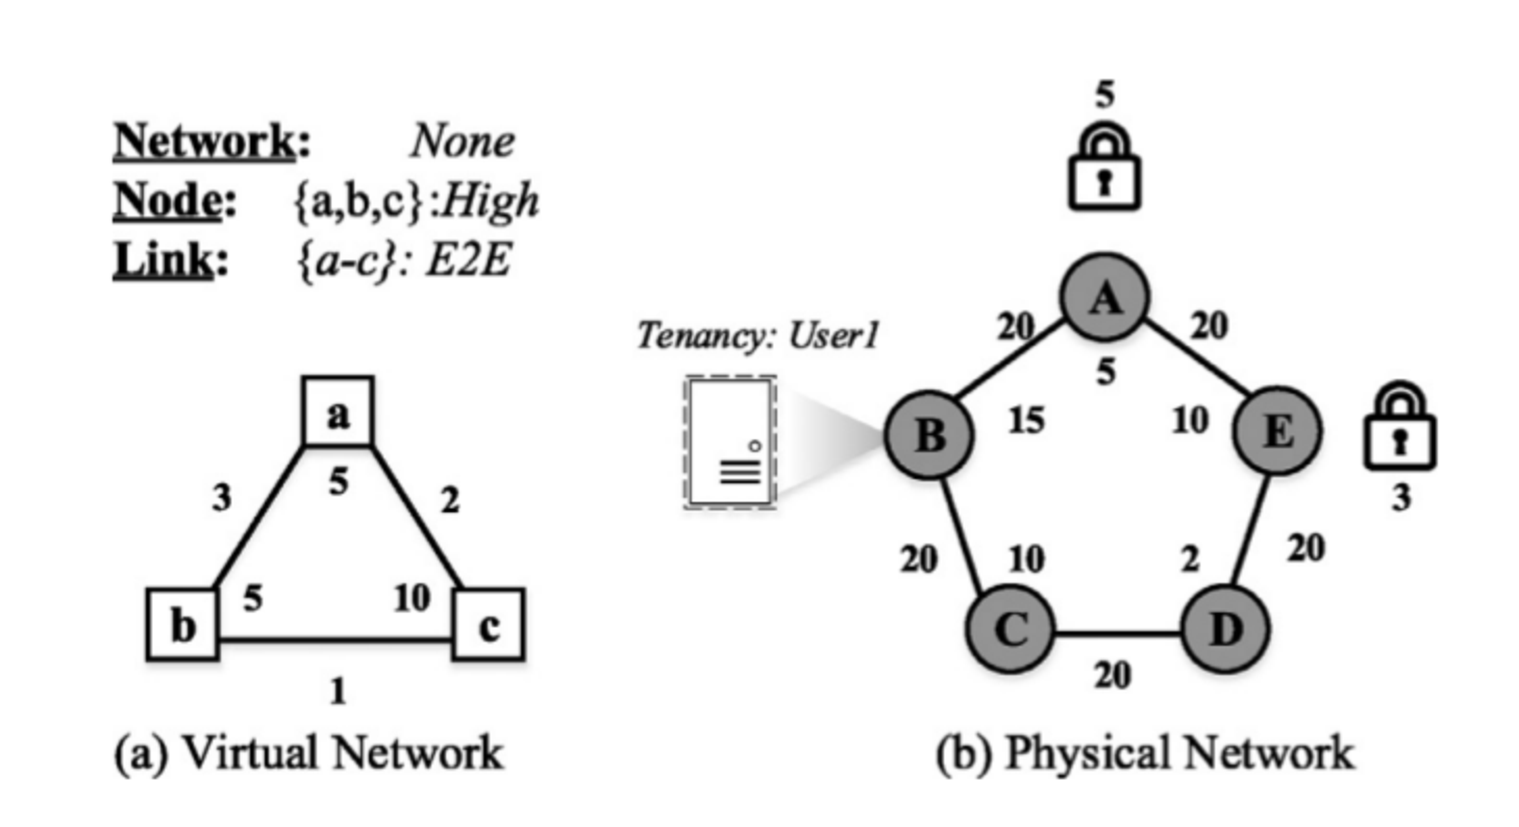
\includegraphics[width=0.8\textwidth]{SVNR.pdf}\newline
\end{center}
Nun wird ein vier-stufiges Pre-Processing durchgef?hrt, um die Berechnung der optimalen Abbildung der VNRs zu vereinfachen. Hierbei werden als ersten die Standardanforderungen der virtuellen Knoten mit den zu Verf?gung stehenden Kapazit?en der physischen Knoten verglichen. Sollten physische Knoten bestimmte Anforderungen nicht erf?llen, werden sie aus der Berechung ausgeschlossen. Der zweite Schritt ist dem"`Network plan"'gewidmet. Sollte ein physischer Knoten, welcher den Anforderungen des"`Network plan"'nicht gen?gt sich in einem Kandidaten-Netzwerk befinden, wird das Subnetz aus den Berechnungen ausgeschlossen. Im dritten Schritt werden die Sicherheitsanforderungen der einzelnen Knoten betrachtet und nicht entsprechende physischen Knoten werden abermals entfernt. Der letzte Schritt widmet sich den Sicherheitsanforderungen aus dem"`Link plan"'und streicht Links aus den weiteren Berrechnungen, welche den Verschl?sselungsanforderungen der virtuellen Links nicht gen?ge tun.\newline
\begin{center}
	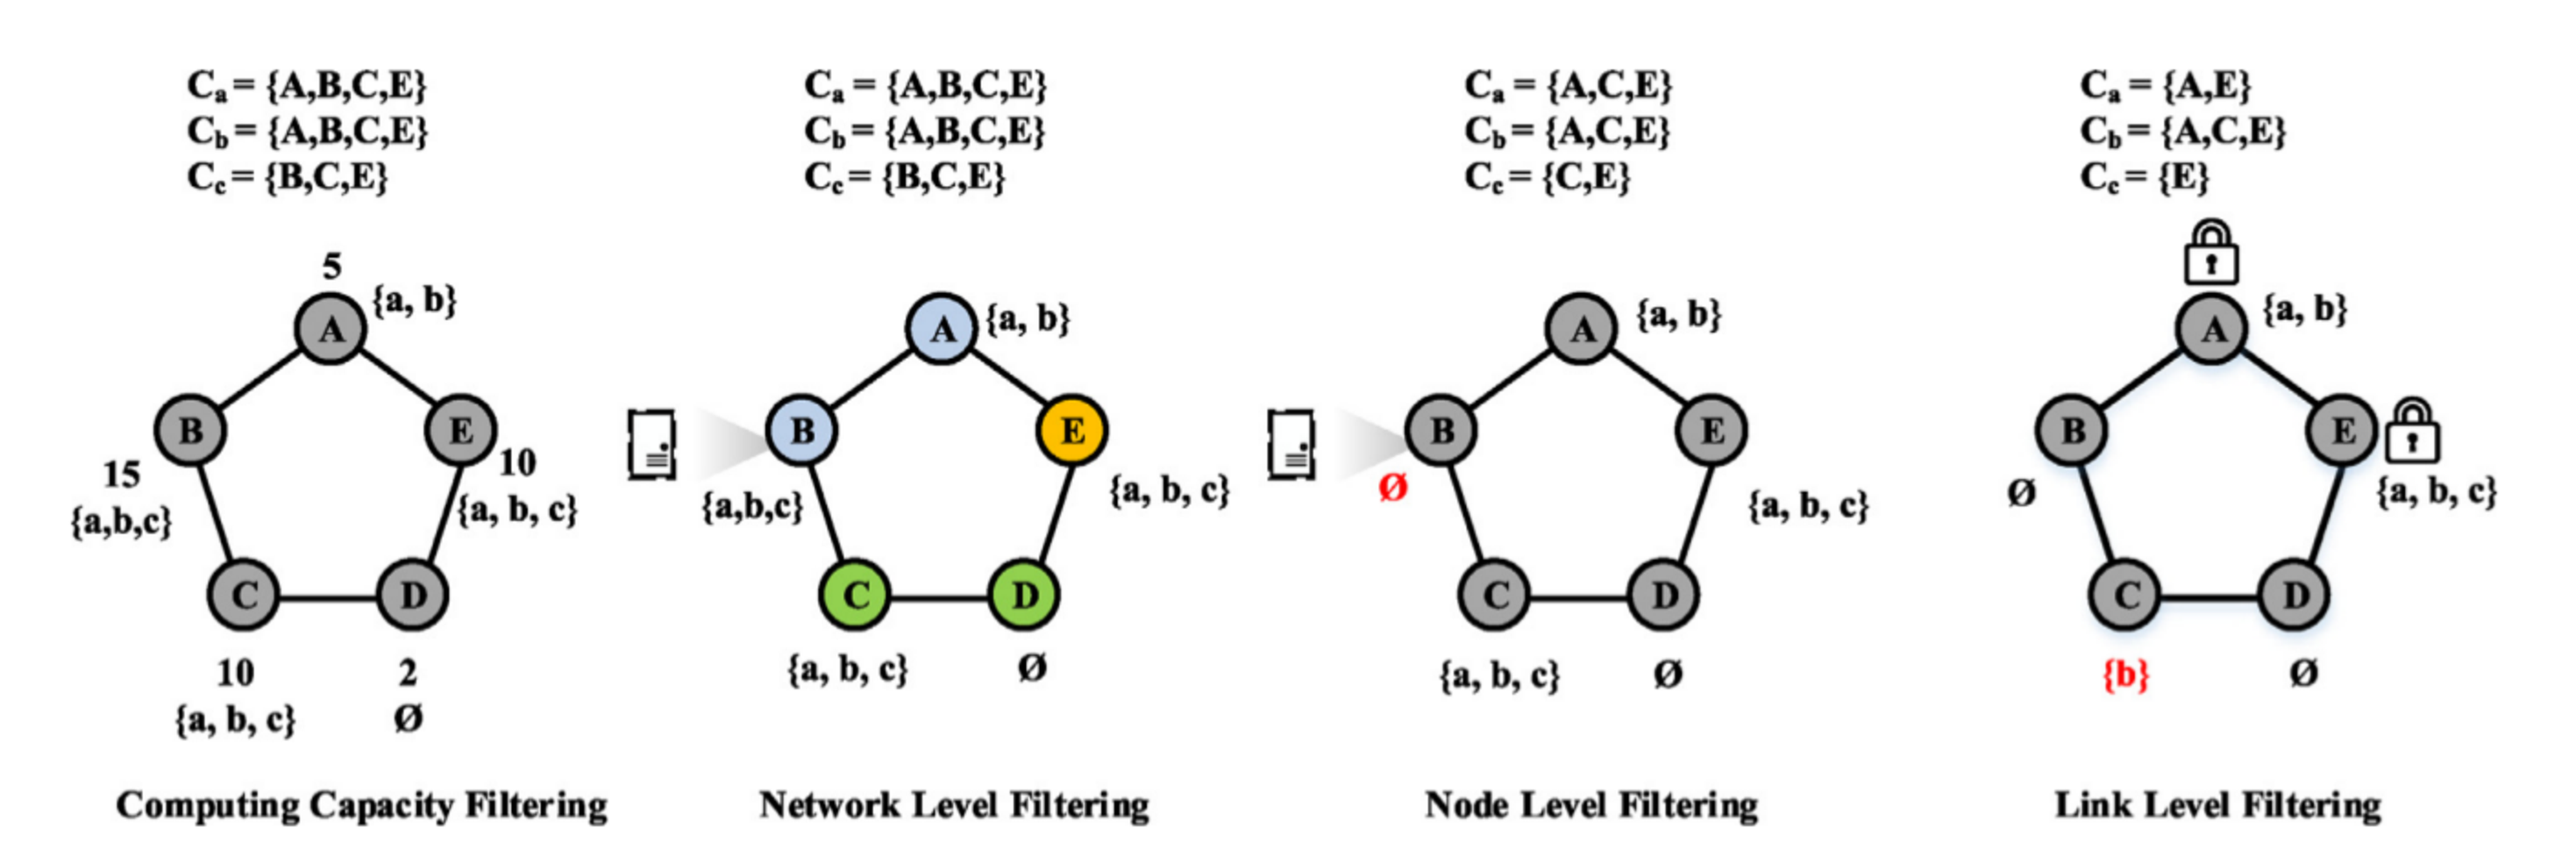
\includegraphics[width=1\textwidth]{pre-processing.pdf}\newline
\end{center}
Mit den aus dem Pre-Processing gewonnen Information bildet man nun einen Hilsgraphen, welcher die ?brig gebliebenen M?glichkeiten der Einbettung zeigt.\newline
\begin{center}
	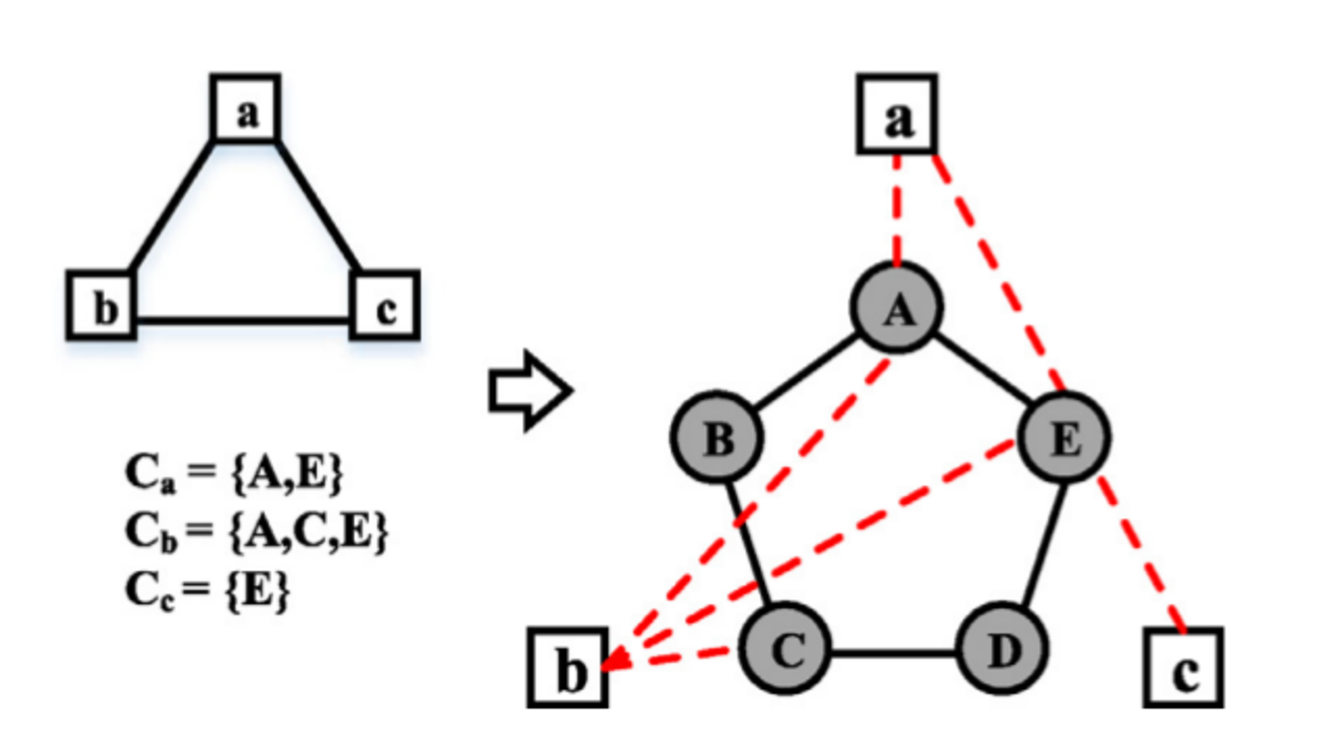
\includegraphics[width=0.6\textwidth]{auxgraph.pdf}\newline 
\end{center}
Dieses Pre-Processing reduziert das SVNE-Problem auf ein"`multi-commodity-flow"'Problem [mit einem Wert (Rohstoff?) pro Link]. \cite{MCF}
Im weiteren Vorgehen werden nun zwei F?le unterschieden."`Path-splitting", im weiteren SVNE-PS und"`no-path-splitting", im weitern SVNE-NPS, sind zus?zliche Sicherheitsvorgaben, welche im Vorfeld definiert werden m?ssen, um die Wahl des Algorithmus zu erm?glichen. Sollte SVNE-PS gew?lt werden, beziehen sich die Gleichungen nur auf die Erf?llung der geforderten Attribute.
Sollte SVNE-NPS gew?lt werden, werden die f?r Link-Abbildungen verantwortlichen Gleichungen ersetzt.\newline
\begin{center}
	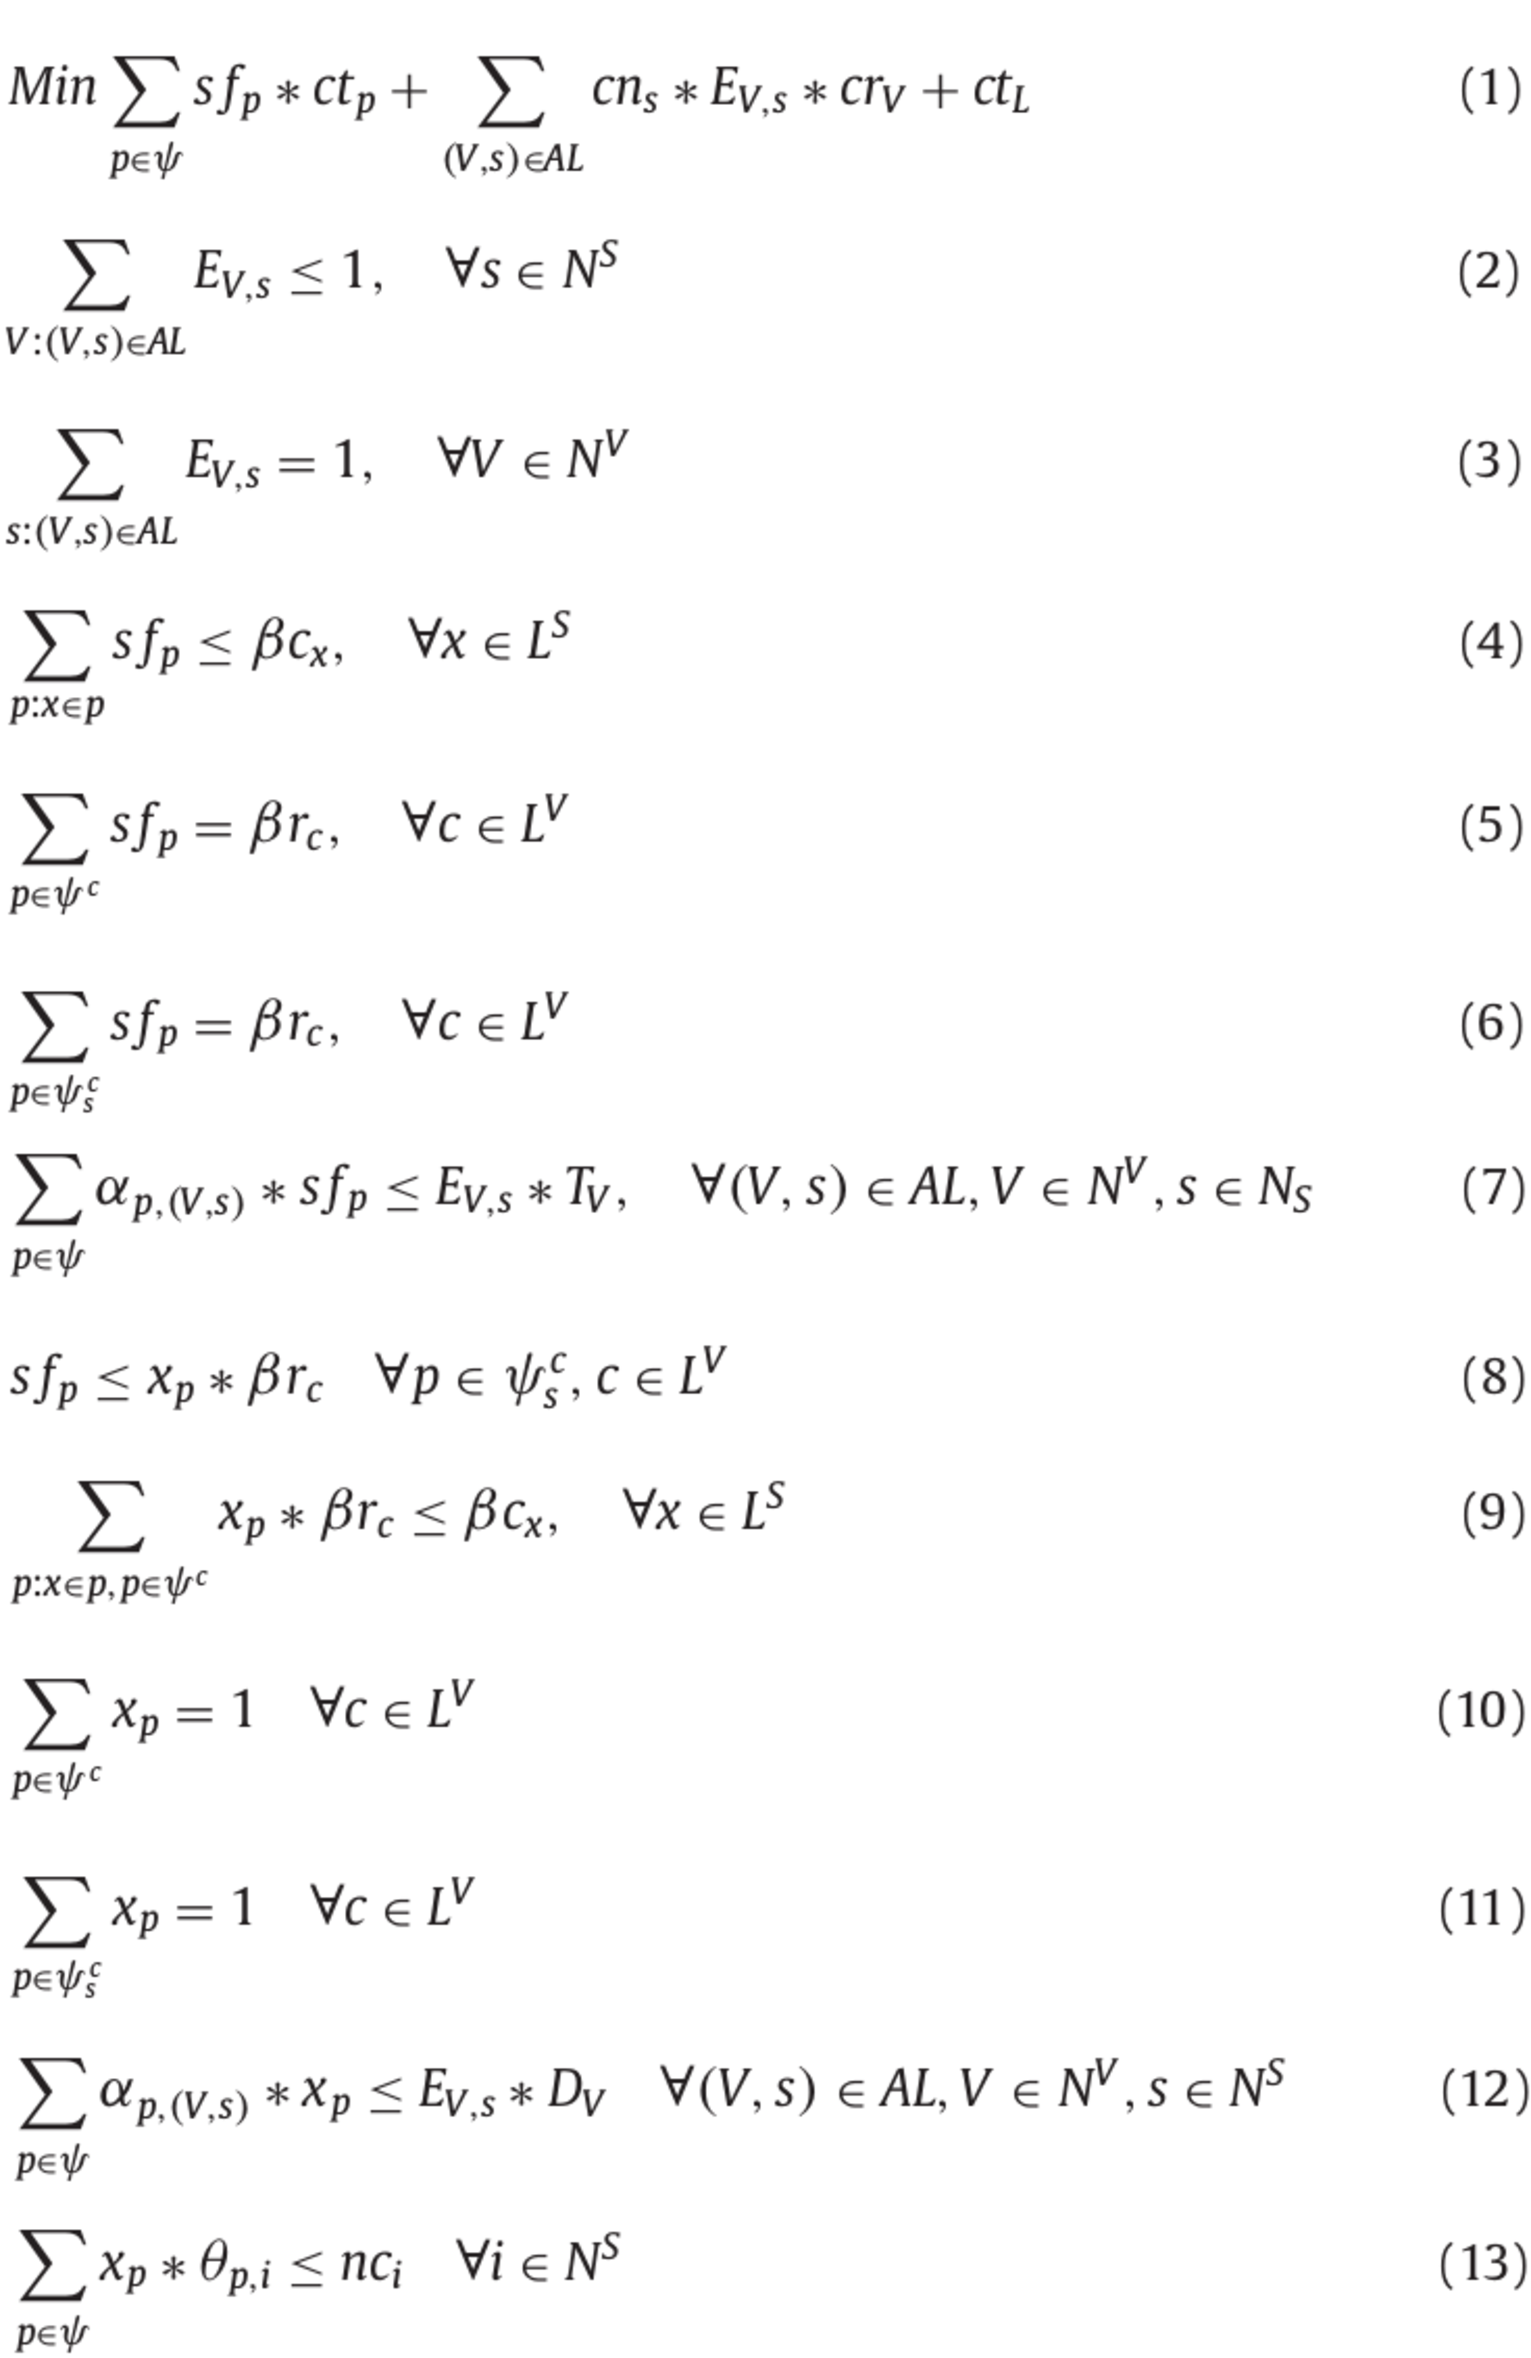
\includegraphics[width=1\textwidth]{algo.pdf}\newline
\end{center}
\begin{center}
	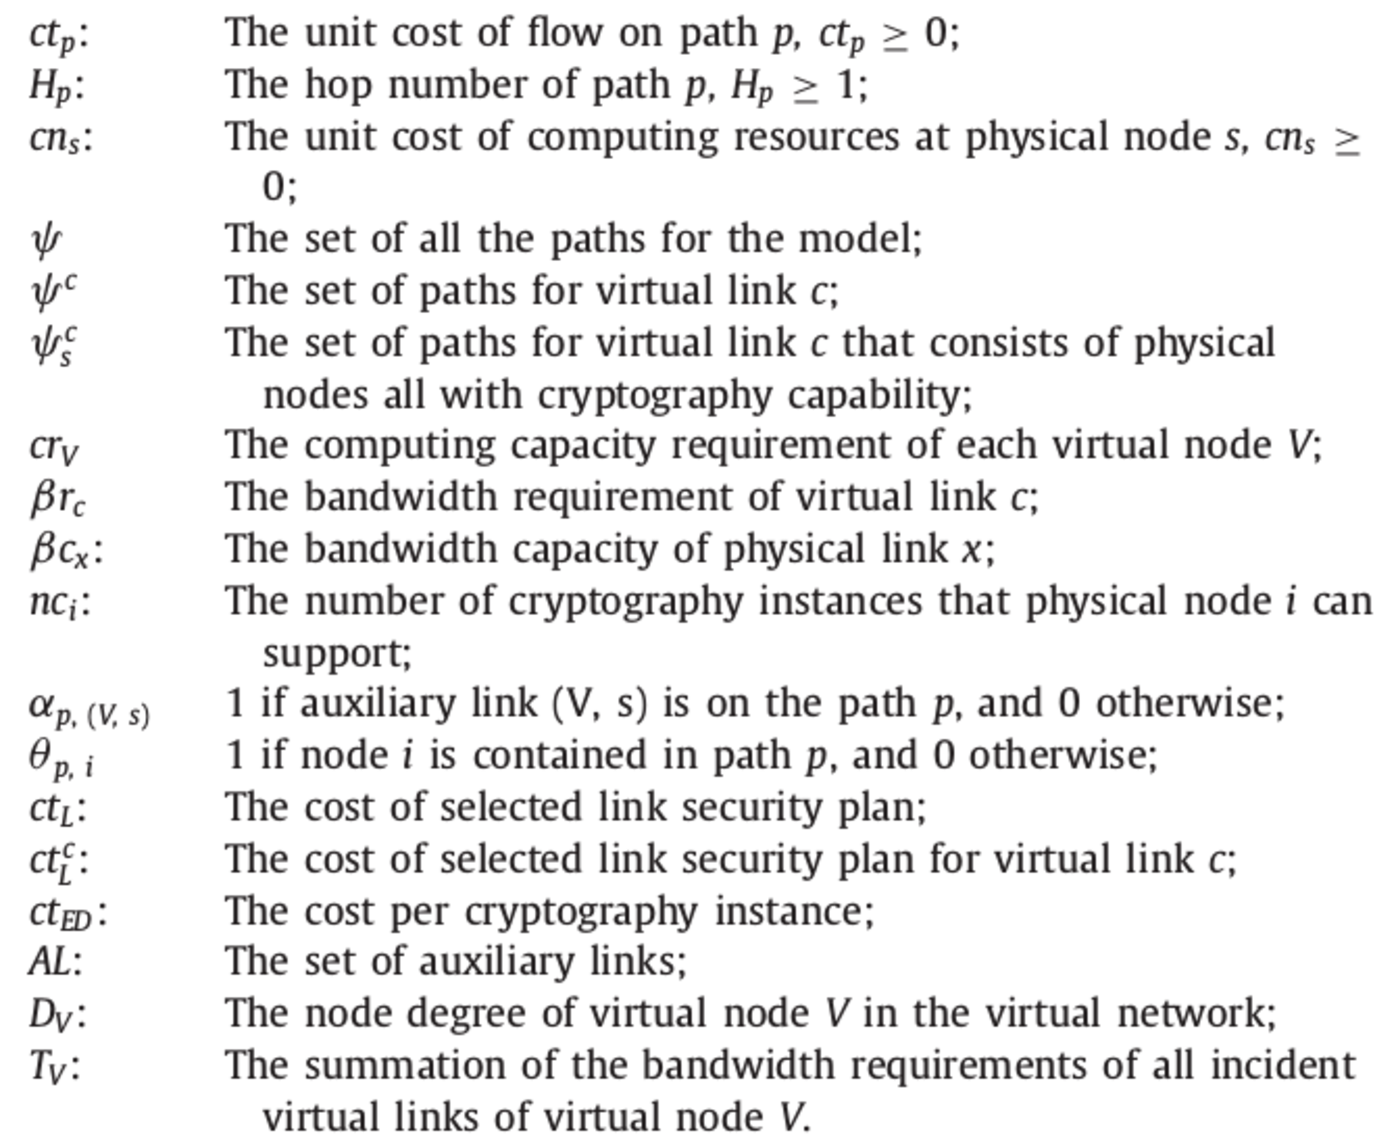
\includegraphics[width=1\textwidth]{notations.pdf}\newline
	\newline
	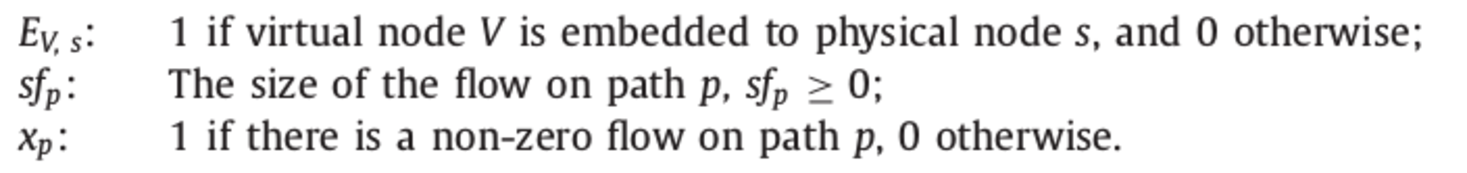
\includegraphics[width=1\textwidth]{variables.pdf}\newline
\end{center}

Fehlt: Kurze Beschreibung der Punkte 1-13\newline

Die Berechnungen wurden mittels induktiver logischer Programmierung unter Verwendung von CPLEX\cite{CPLEX} und durch k-shortest-path anhand aller abzubildenden Elemente limitiert.
F?r die Testumgebungen wurden zuf?lig erzeugte VNRs mit 2 bis 10 Knoten und halbsovielen Links erzeugt. Auch die Rechenkapazit? wie Bandbreite wurden durch Zufallsgeneratoren mit Werten im Bereich von 1 bis 10 gew?lt und verteilt. Die Anzahl der VNRs betr?t einer Poisson-Verteilung nach einen Durchschnitt von 4 VNR pro 100 Zeiteinheiten, mit einer jeweiligen durchschnittlichen Einsatzzeit von 1000 Zeiteinheiten.

Die zugrundeliegenden physischen Netze wurden ebenfalls zuf?lig erzeugt und beinhalteten 10 bis 50 Knoten, sowie halbsoviele Links. Die Rechen- sowie Bandbreiten-Kapazit?en wurden gleichm?ig verteilt und enthielten Werte zwischen 1 und 50. Die Verschl?sselungskapazit?en der Knoten  wurde ?ber die gesamte Testreihe ebenfalls gleichm?ig verteilt.

Die folgende Statisk zeigt einen Durchschnittsvergleich zwischen dem, als Standard gew?lten, VNE-Algorithmus\cite{Std} und den beiden SVNE-Varianten PS und NPS. Dazu sei gesagt dass s?tliche Algorithmen ihre Berechnungen anhand des Hilfsgraphen durchgef?hrt haben und durch k=3 bzw. k=4 limitiert wurden.\newline
\begin{center}
	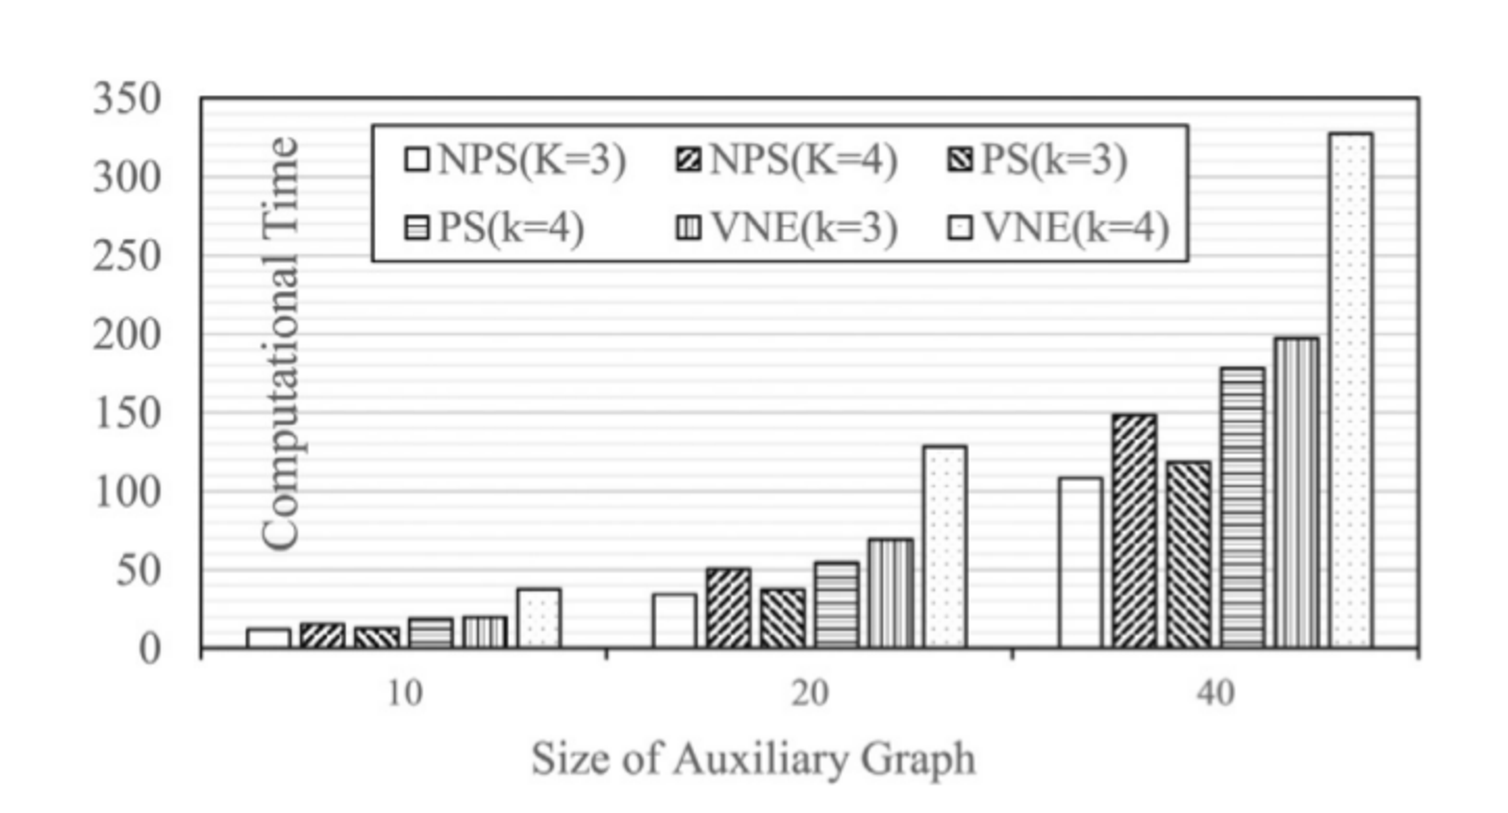
\includegraphics[width=0.8\textwidth]{statistic.pdf}\newline
\end{center}
Man sieht  hier einen deutlichen Zeitvorsprung von PS und NPS gegen?ber dem Standard-Algorithmus. Da hier jedoch auch der Standard-Algorithmus vom Pre-Processing profitiert, w?e ein Vergleich, welcher die Dauer des Pre-Processings mit aufnimmt und den Standard-Algorithmus ohne Pre-Processing arbeiten lie?, anschaulicher und aussagekr?tiger.
Dennoch ist ein Punkt durchaus ?berraschend und bemerkenswert: Der Standard-Algorithmus ben?tigt deutlich l?ger, obwohl er keine Sicherheitsaspekte mitbeurteilt, im Gegenzug zu seinen Kontrahenten.

In welchem Komplexit?sbereich sich das Pre-Processing befindet wird hier leider nicht erw?nt.


\subsection{Ansatz 2}

Im zweiten Ansatz widmen wir uns dem Modell aus \cite{algo2}. Dieser Ansatz arbeitet mit abstrakten Sicherheitslevels. Im Folgenden werden zwar Skalare hierf?r verwendet, was allerdings nicht zwingend so vorgesehen ist. Stattdessen w?e eine Verwendung komplexerer Sicherheitsvektoren m?glich, welche bei weitem detailliertere Sicherheitsmerkmale  beschreiben k?nnten. Des weiteren verf?gt jeder physische wie auch virtuelle Knoten ?ber zwei Sicherheitswerte: Anforderungslevel und (eigenes) Sicherheitslevel. Der Anforderungslevel definiert das Minimum-Level des Gegen?bers, der Sicherheitslevel definiert die eigenen gew?nschten Sicherheitsmerkmale. Virtuelle Links verf?gen ?ber Anforderungslevels, physische Links nur ?ber Sicherheitslevels. Die vorausgesetzten Basisanforderungen, welchen alle VNRs unterliegen, beschr?ken sich auf 4 Regeln, welche mittels der zuvor genannten Merkmale umgesetzt werden:
\begin{itemize}
\item Ein physischer Knoten sollte einen Sicherheitslevel garantieren, 
   der h?her ist als die Anforderungen der darauf abzubildenden
   virtuellen Knoten.

\item Der Sicherheitslevel des virtuellen Knotens sollte h?her sein, 
   als das Anforderungslevel des physichen Knotens.

\item Alle virtuellen Knoten, welche auf den selben physischen Knoten
   abgebildet werden, sollten ?ber einen ausreichenden Sicherheitslevel
   verf?gen.

\item Der Anforderungslevel des virtuellen Links sollte stets niedriger
   sein, als das Sicherheitslevel des physischen Links.
\end{itemize}%\end{listing}

\begin{center}
	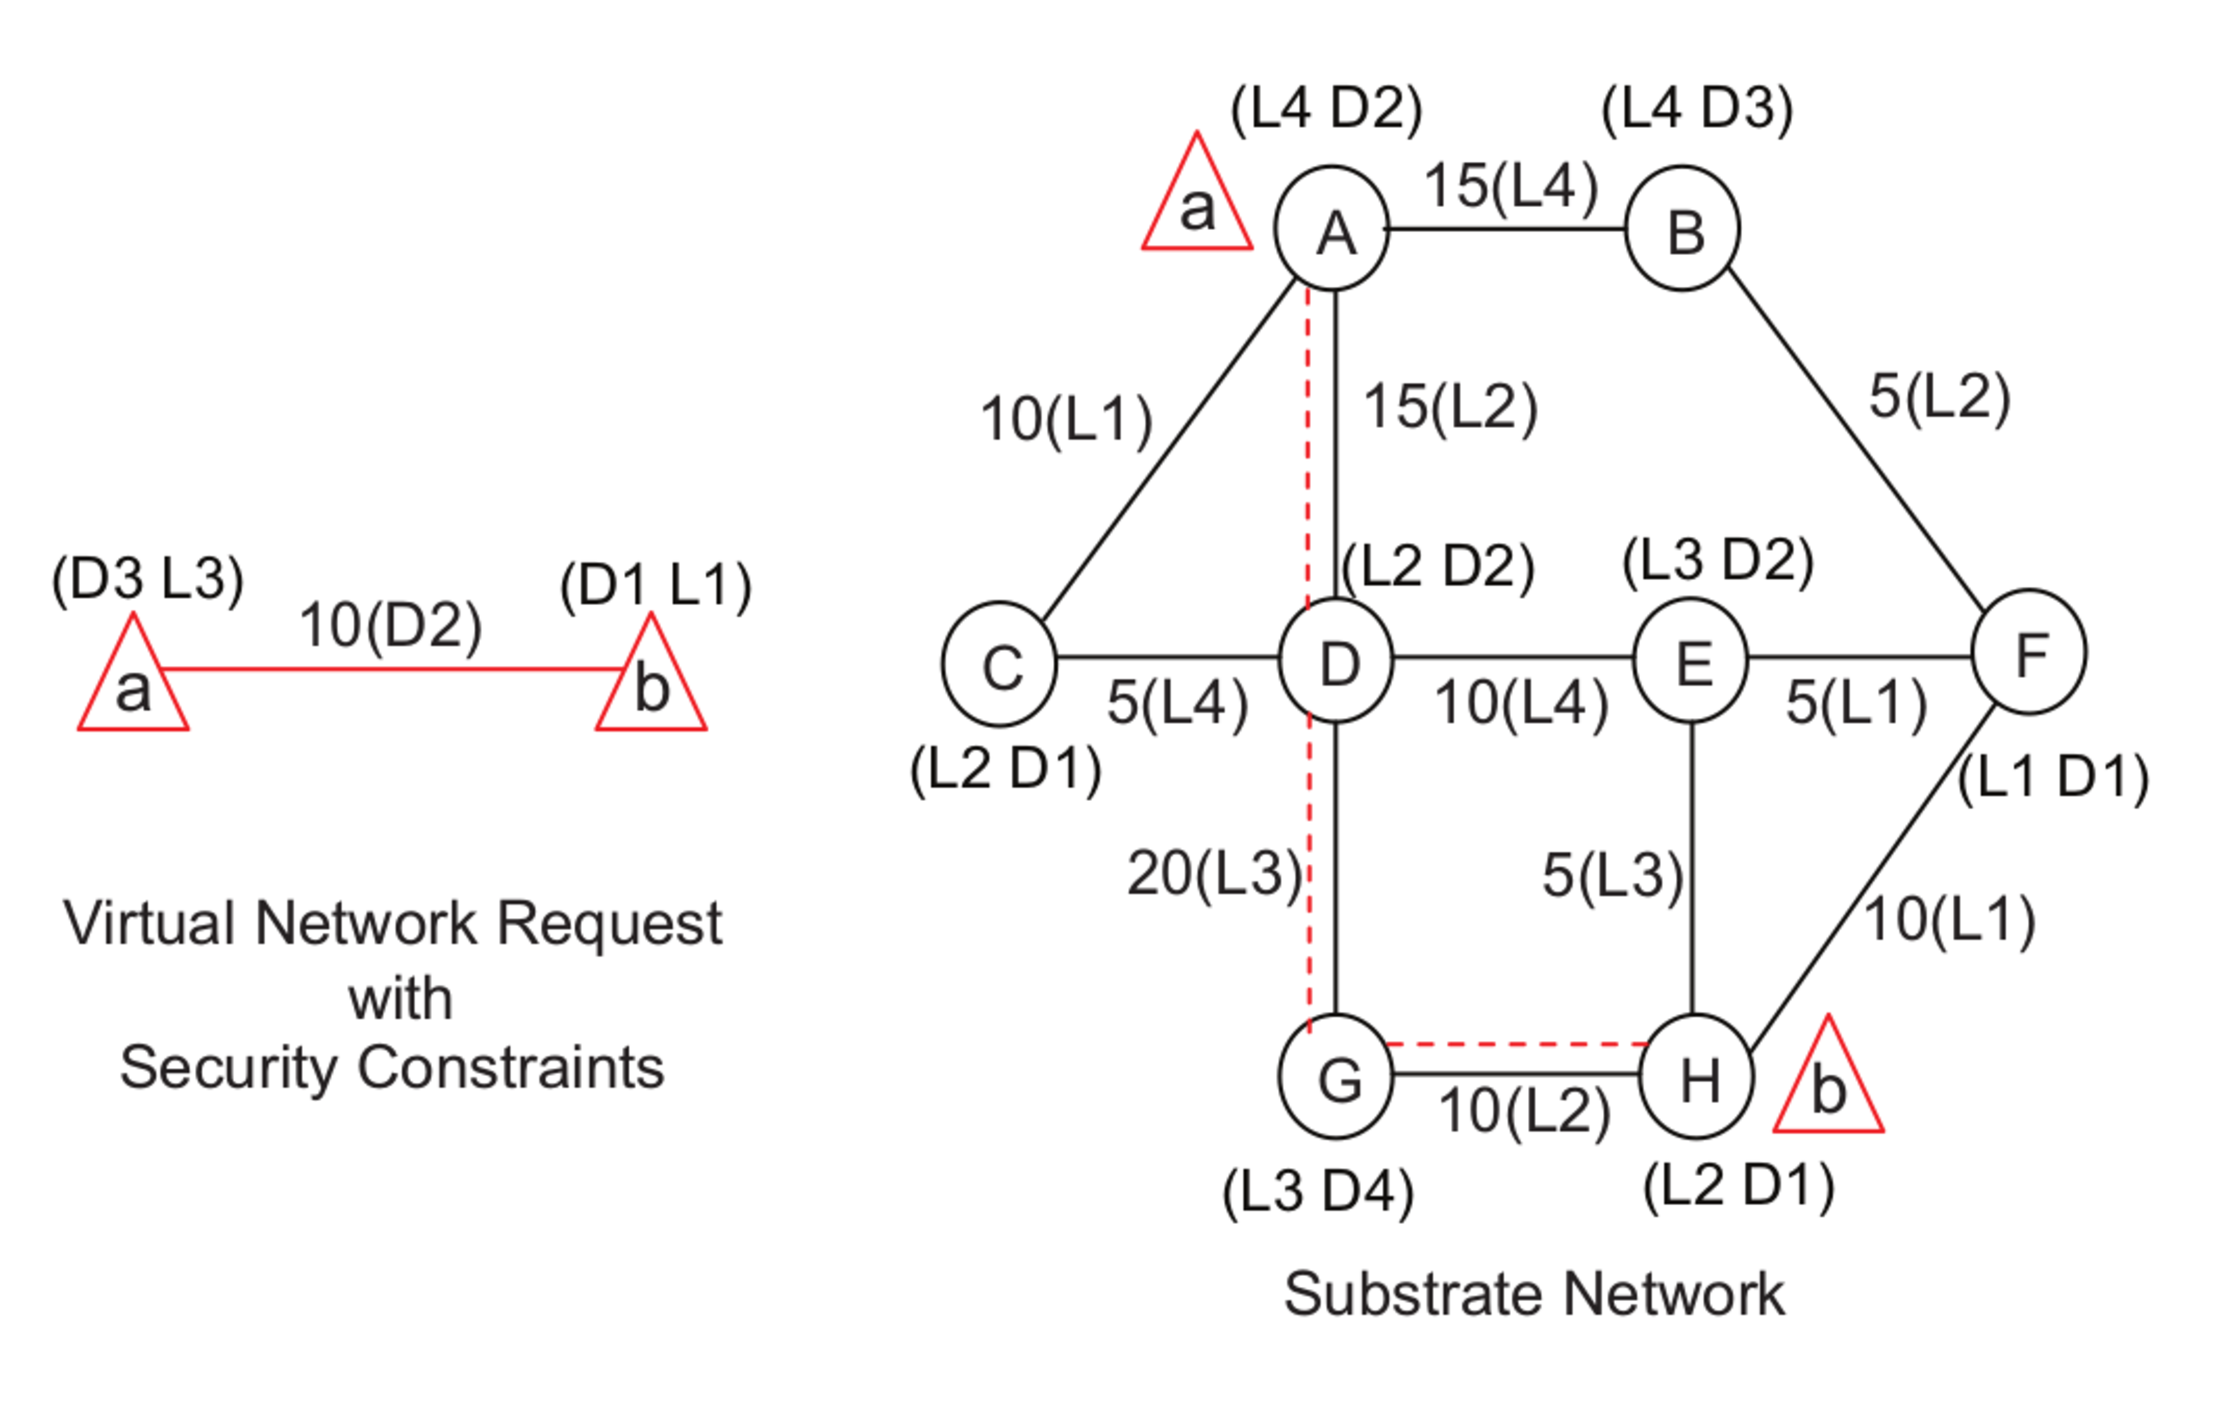
\includegraphics[width=0.8\textwidth]{algo2graph.pdf}\newline
\end{center}
Wie man in Abbildung X sieht, werden auch bei diesem Modell VNRs und physische Netze in ungerichtete Graphen transformiert. Die in Klammern gestellten Parameter beschreiben Anforderungslevel(D) und Sicherheitslevel(L). Die hier durchgef?hrte Abbildung ber?cksichtigt nicht nur die Sicherheitsanforderungen aller Parteien unter Ber?cksichtigung der Basisanforderungen, sondern achtet zus?zlich noch auf Kostenminimierung. Insgesamt existieren drei Abbildungsm?glichkeiten, die gew?lte ist jedoch die g?nstigste, unter dem Aspekt keine Sicherheitsresourcen zu verschwenden. Dieser VNR h?te auch auf EDGH abgebildet werden k?nnen, wobei der Link ED ?ber einen Sicherheitslevel verf?gt, welcher h?her als n?tig ist. W?rde dies nicht beachtet werden, k?nnte es zu unn?tigen Engp?sen bei der Behandlung von VNRs mit h?heren Anforderungslevels kommen. Um ein solches Verhalten zu erreichen, wurden zus?zlich Kosten- und Nutzen-Funktionen in die Berechnung integriert.
\begin{center}
	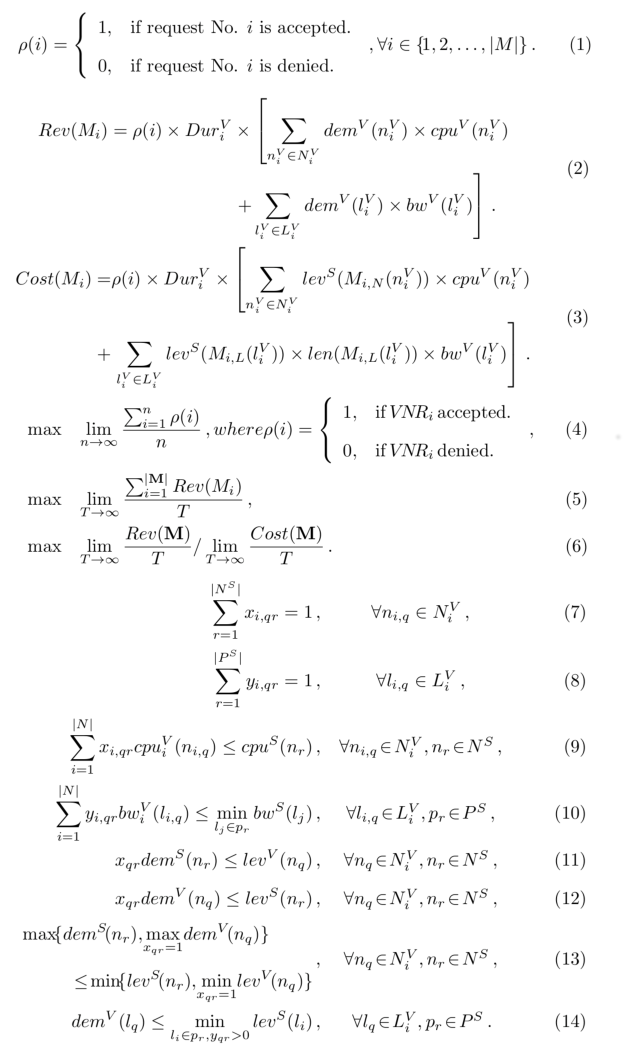
\includegraphics[width=0.8\textwidth]{algo2.pdf}\newline
\end{center}

Fehlt: Kurze Beschreibung der Punkte 1-16

Das außergewöhnliche bei diesem Ansatz ist die Verwendung zweier unterschiedlicher Algorithmen, welche sich gegenseitig ergänzen: uSAV und cSAV.
\begin{itemize}
	\item uSAV \newline
	uSAV, der unkooridinierte zwei-Phasen-Algorithmus, behandelt Knoten- und Link-Abbildungen getrennt voneinander. Dementsprechend liegt die Schwäche von uSAV in der Abbildung von non-splittable-links. uSAV ist ein terminierender Algorithmus, welcher die Abbildung der Knoten priorisiert und dahingehend ein sehr gutes Ergebnis mit wenig Aufwand erzielt. Jedoch kann es, durch die Priorisierung der Knoten, zu hohen Kosten bei der Link-Abbildung kommen.

	\item cSAV \newline
	cSAV, der koordinierte Algorithmus, behandelt Knoten und Links gemeinsam, und kann zur Optimierung, des bereits von uSAV gelieferten Ergebnisses verwendet werden. cSAV liefert zwar optimalere Ergebnisse als uSAV, benötigt aber auch mehr Zeit. Hier muss Zeitaufwand mit gelieferter Leistung abgewogen werden.

\end{itemize} 

Beide Varianten nutzen die selben Heuristiken ((und Sub-Algorithmen)). Der Author schlägt für ideale Ergebnisse eine kombinierte Benutzung der beiden Varianten vor.

\begin{center}
uSAV\newline
	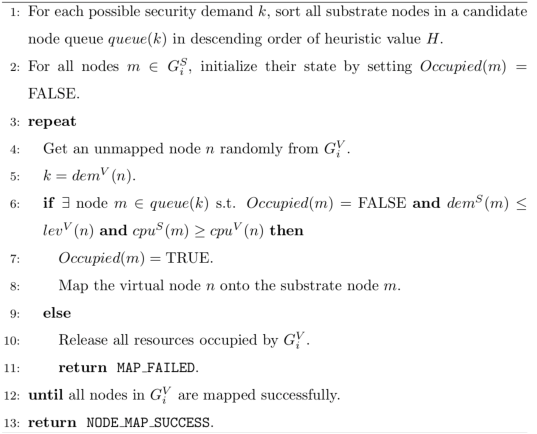
\includegraphics[width=0.8\textwidth]{usav.pdf}\newline
\end{center}
\newpage
\begin{center}
cSAV\newline
	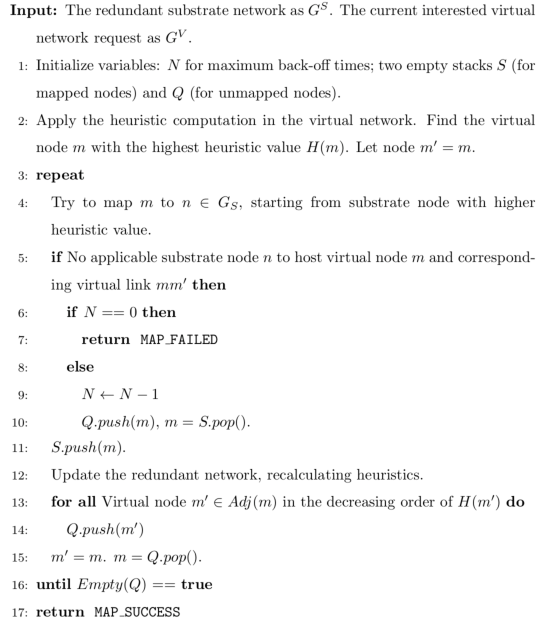
\includegraphics[width=0.8\textwidth]{csav.pdf}\newline
\end{center}
\newpage
\begin{center}
Sub-Algorithmus 1: Knoten-Abbildungen\newline
	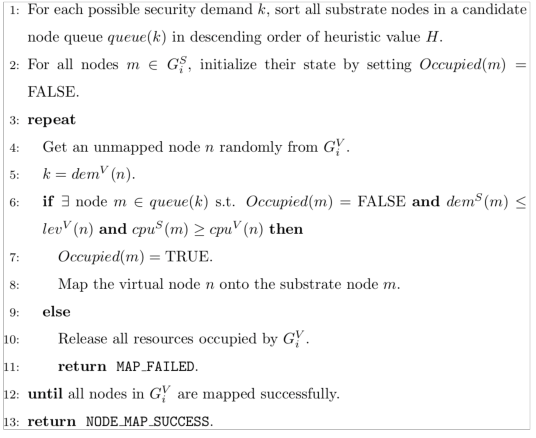
\includegraphics[width=0.8\textwidth]{nodemapping.pdf}\newline
\end{center}
\newpage
\begin{center}
Sub-Algorithmus 2: Link-Abbildungen\newline
	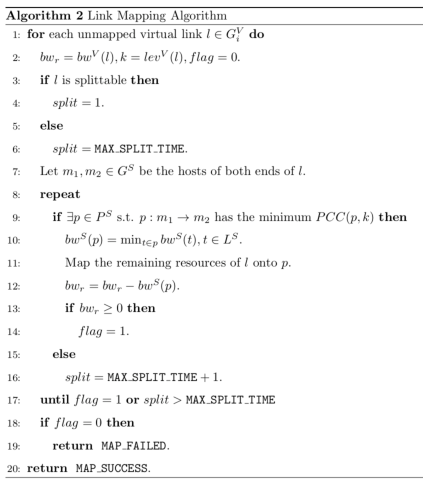
\includegraphics[width=0.8\textwidth]{linkmapping.pdf}\newline
\end{center}

Die Testumgebung dieses Ansatzes wurde mittels GT-ITM-Tool cite-missing! erstellt. 

Die physischen Netze wurden in der Größenordnung eines mittleres ISP angesetzt, und betrugen 100 Knoten und 500 Links. Die Bandbreite und Rechenkapazität wurden, wie auch im vorherigen Ansatz, gleichmäßig verteilt und betrugen Werte zwischen 50 und 100. Die abstrakten Sicherheitslevels der physischen Elemente wurden zwischen 0 und 4 gleichmäßig verteilt. Die Anforderungslevels wurden ebenfalls aus dem Bereich 0-4 gewählt, und so verteilt, dass kein physisches Element ein höheres Anforderungslevel als Sicherheitslevel besitzt.

Die VNRs beinhalteten 2 bis 20 Knoten sowie halbsoviele Links. Die Bandbreite- und Rechenkapazitäts-Forderungen wurden zwischen 0 und 50 gewählt und ebenfalls gleichmäßig verteilt.
Die zeitlichen Parameter wurden auf durchschnittlich (Poisson-Verteilung) 5 Anforderungen pro 100 Zeiteinheiten begrenzt. Die Verwendungszeit eines VNRs folgt einer Exponential-Verteilung und betrugt im Durchschnitt 500 Zeiteinheiten. Eine einzelne Simulation erhielt 1500 VNRs und dauerte 30000 Zeiteinheiten.

Als Vergleichswert wurde der Algorithmus aus cite-6-missingverwendet.




\subsection{Vergleich}
\label{subsec:svne_vergleich}



\section{Ungel?ste Probleme}
\label{sec:offenefragen}

\section{Schlussfolgerung und Ausblick}
\label{sec:schluss}
Frage: Auf welcher Ebene wird virtualisiert? Auf IP-Ebene? Was ist dann aber mit IP-Support-Protokollen (ARP)? Oder nicht-IP-Protokollen? Will ich ein Netzwerk virtualisieren, oder nur den IP-Verkehr? Verkapselung f?hrt zu Leistungseinbu?n. \cite{cabuk2007towards}



\bibliography{literatur}{}

\end{document}



